\documentclass{article} % For LaTeX2e
\usepackage{iclr2022_conference,times}
\usepackage{svg}
\usepackage{hyperref}
\svgpath{{Figs/}}
% Optional math commands from https://github.com/goodfeli/dlbook_notation.
%%%%% NEW MATH DEFINITIONS %%%%%

\usepackage{amsmath,amsfonts,bm}

% Mark sections of captions for referring to divisions of figures
\newcommand{\figleft}{{\em (Left)}}
\newcommand{\figcenter}{{\em (Center)}}
\newcommand{\figright}{{\em (Right)}}
\newcommand{\figtop}{{\em (Top)}}
\newcommand{\figbottom}{{\em (Bottom)}}
\newcommand{\captiona}{{\em (a)}}
\newcommand{\captionb}{{\em (b)}}
\newcommand{\captionc}{{\em (c)}}
\newcommand{\captiond}{{\em (d)}}

% Highlight a newly defined term
\newcommand{\newterm}[1]{{\bf #1}}


% Figure reference, lower-case.
\def\figref#1{figure~\ref{#1}}
% Figure reference, capital. For start of sentence
\def\Figref#1{Figure~\ref{#1}}
\def\twofigref#1#2{figures \ref{#1} and \ref{#2}}
\def\quadfigref#1#2#3#4{figures \ref{#1}, \ref{#2}, \ref{#3} and \ref{#4}}
% Section reference, lower-case.
\def\secref#1{section~\ref{#1}}
% Section reference, capital.
\def\Secref#1{Section~\ref{#1}}
% Reference to two sections.
\def\twosecrefs#1#2{sections \ref{#1} and \ref{#2}}
% Reference to three sections.
\def\secrefs#1#2#3{sections \ref{#1}, \ref{#2} and \ref{#3}}
% Reference to an equation, lower-case.
\def\eqref#1{equation~\ref{#1}}
% Reference to an equation, upper case
\def\Eqref#1{Equation~\ref{#1}}
% A raw reference to an equation---avoid using if possible
\def\plaineqref#1{\ref{#1}}
% Reference to a chapter, lower-case.
\def\chapref#1{chapter~\ref{#1}}
% Reference to an equation, upper case.
\def\Chapref#1{Chapter~\ref{#1}}
% Reference to a range of chapters
\def\rangechapref#1#2{chapters\ref{#1}--\ref{#2}}
% Reference to an algorithm, lower-case.
\def\algref#1{algorithm~\ref{#1}}
% Reference to an algorithm, upper case.
\def\Algref#1{Algorithm~\ref{#1}}
\def\twoalgref#1#2{algorithms \ref{#1} and \ref{#2}}
\def\Twoalgref#1#2{Algorithms \ref{#1} and \ref{#2}}
% Reference to a part, lower case
\def\partref#1{part~\ref{#1}}
% Reference to a part, upper case
\def\Partref#1{Part~\ref{#1}}
\def\twopartref#1#2{parts \ref{#1} and \ref{#2}}

\def\ceil#1{\lceil #1 \rceil}
\def\floor#1{\lfloor #1 \rfloor}
\def\1{\bm{1}}
\newcommand{\train}{\mathcal{D}}
\newcommand{\valid}{\mathcal{D_{\mathrm{valid}}}}
\newcommand{\test}{\mathcal{D_{\mathrm{test}}}}

\def\eps{{\epsilon}}


% Random variables
\def\reta{{\textnormal{$\eta$}}}
\def\ra{{\textnormal{a}}}
\def\rb{{\textnormal{b}}}
\def\rc{{\textnormal{c}}}
\def\rd{{\textnormal{d}}}
\def\re{{\textnormal{e}}}
\def\rf{{\textnormal{f}}}
\def\rg{{\textnormal{g}}}
\def\rh{{\textnormal{h}}}
\def\ri{{\textnormal{i}}}
\def\rj{{\textnormal{j}}}
\def\rk{{\textnormal{k}}}
\def\rl{{\textnormal{l}}}
% rm is already a command, just don't name any random variables m
\def\rn{{\textnormal{n}}}
\def\ro{{\textnormal{o}}}
\def\rp{{\textnormal{p}}}
\def\rq{{\textnormal{q}}}
\def\rr{{\textnormal{r}}}
\def\rs{{\textnormal{s}}}
\def\rt{{\textnormal{t}}}
\def\ru{{\textnormal{u}}}
\def\rv{{\textnormal{v}}}
\def\rw{{\textnormal{w}}}
\def\rx{{\textnormal{x}}}
\def\ry{{\textnormal{y}}}
\def\rz{{\textnormal{z}}}

% Random vectors
\def\rvepsilon{{\mathbf{\epsilon}}}
\def\rvtheta{{\mathbf{\theta}}}
\def\rva{{\mathbf{a}}}
\def\rvb{{\mathbf{b}}}
\def\rvc{{\mathbf{c}}}
\def\rvd{{\mathbf{d}}}
\def\rve{{\mathbf{e}}}
\def\rvf{{\mathbf{f}}}
\def\rvg{{\mathbf{g}}}
\def\rvh{{\mathbf{h}}}
\def\rvu{{\mathbf{i}}}
\def\rvj{{\mathbf{j}}}
\def\rvk{{\mathbf{k}}}
\def\rvl{{\mathbf{l}}}
\def\rvm{{\mathbf{m}}}
\def\rvn{{\mathbf{n}}}
\def\rvo{{\mathbf{o}}}
\def\rvp{{\mathbf{p}}}
\def\rvq{{\mathbf{q}}}
\def\rvr{{\mathbf{r}}}
\def\rvs{{\mathbf{s}}}
\def\rvt{{\mathbf{t}}}
\def\rvu{{\mathbf{u}}}
\def\rvv{{\mathbf{v}}}
\def\rvw{{\mathbf{w}}}
\def\rvx{{\mathbf{x}}}
\def\rvy{{\mathbf{y}}}
\def\rvz{{\mathbf{z}}}

% Elements of random vectors
\def\erva{{\textnormal{a}}}
\def\ervb{{\textnormal{b}}}
\def\ervc{{\textnormal{c}}}
\def\ervd{{\textnormal{d}}}
\def\erve{{\textnormal{e}}}
\def\ervf{{\textnormal{f}}}
\def\ervg{{\textnormal{g}}}
\def\ervh{{\textnormal{h}}}
\def\ervi{{\textnormal{i}}}
\def\ervj{{\textnormal{j}}}
\def\ervk{{\textnormal{k}}}
\def\ervl{{\textnormal{l}}}
\def\ervm{{\textnormal{m}}}
\def\ervn{{\textnormal{n}}}
\def\ervo{{\textnormal{o}}}
\def\ervp{{\textnormal{p}}}
\def\ervq{{\textnormal{q}}}
\def\ervr{{\textnormal{r}}}
\def\ervs{{\textnormal{s}}}
\def\ervt{{\textnormal{t}}}
\def\ervu{{\textnormal{u}}}
\def\ervv{{\textnormal{v}}}
\def\ervw{{\textnormal{w}}}
\def\ervx{{\textnormal{x}}}
\def\ervy{{\textnormal{y}}}
\def\ervz{{\textnormal{z}}}

% Random matrices
\def\rmA{{\mathbf{A}}}
\def\rmB{{\mathbf{B}}}
\def\rmC{{\mathbf{C}}}
\def\rmD{{\mathbf{D}}}
\def\rmE{{\mathbf{E}}}
\def\rmF{{\mathbf{F}}}
\def\rmG{{\mathbf{G}}}
\def\rmH{{\mathbf{H}}}
\def\rmI{{\mathbf{I}}}
\def\rmJ{{\mathbf{J}}}
\def\rmK{{\mathbf{K}}}
\def\rmL{{\mathbf{L}}}
\def\rmM{{\mathbf{M}}}
\def\rmN{{\mathbf{N}}}
\def\rmO{{\mathbf{O}}}
\def\rmP{{\mathbf{P}}}
\def\rmQ{{\mathbf{Q}}}
\def\rmR{{\mathbf{R}}}
\def\rmS{{\mathbf{S}}}
\def\rmT{{\mathbf{T}}}
\def\rmU{{\mathbf{U}}}
\def\rmV{{\mathbf{V}}}
\def\rmW{{\mathbf{W}}}
\def\rmX{{\mathbf{X}}}
\def\rmY{{\mathbf{Y}}}
\def\rmZ{{\mathbf{Z}}}

% Elements of random matrices
\def\ermA{{\textnormal{A}}}
\def\ermB{{\textnormal{B}}}
\def\ermC{{\textnormal{C}}}
\def\ermD{{\textnormal{D}}}
\def\ermE{{\textnormal{E}}}
\def\ermF{{\textnormal{F}}}
\def\ermG{{\textnormal{G}}}
\def\ermH{{\textnormal{H}}}
\def\ermI{{\textnormal{I}}}
\def\ermJ{{\textnormal{J}}}
\def\ermK{{\textnormal{K}}}
\def\ermL{{\textnormal{L}}}
\def\ermM{{\textnormal{M}}}
\def\ermN{{\textnormal{N}}}
\def\ermO{{\textnormal{O}}}
\def\ermP{{\textnormal{P}}}
\def\ermQ{{\textnormal{Q}}}
\def\ermR{{\textnormal{R}}}
\def\ermS{{\textnormal{S}}}
\def\ermT{{\textnormal{T}}}
\def\ermU{{\textnormal{U}}}
\def\ermV{{\textnormal{V}}}
\def\ermW{{\textnormal{W}}}
\def\ermX{{\textnormal{X}}}
\def\ermY{{\textnormal{Y}}}
\def\ermZ{{\textnormal{Z}}}

% Vectors
\def\vzero{{\bm{0}}}
\def\vone{{\bm{1}}}
\def\vmu{{\bm{\mu}}}
\def\vtheta{{\bm{\theta}}}
\def\va{{\bm{a}}}
\def\vb{{\bm{b}}}
\def\vc{{\bm{c}}}
\def\vd{{\bm{d}}}
\def\ve{{\bm{e}}}
\def\vf{{\bm{f}}}
\def\vg{{\bm{g}}}
\def\vh{{\bm{h}}}
\def\vi{{\bm{i}}}
\def\vj{{\bm{j}}}
\def\vk{{\bm{k}}}
\def\vl{{\bm{l}}}
\def\vm{{\bm{m}}}
\def\vn{{\bm{n}}}
\def\vo{{\bm{o}}}
\def\vp{{\bm{p}}}
\def\vq{{\bm{q}}}
\def\vr{{\bm{r}}}
\def\vs{{\bm{s}}}
\def\vt{{\bm{t}}}
\def\vu{{\bm{u}}}
\def\vv{{\bm{v}}}
\def\vw{{\bm{w}}}
\def\vx{{\bm{x}}}
\def\vy{{\bm{y}}}
\def\vz{{\bm{z}}}

% Elements of vectors
\def\evalpha{{\alpha}}
\def\evbeta{{\beta}}
\def\evepsilon{{\epsilon}}
\def\evlambda{{\lambda}}
\def\evomega{{\omega}}
\def\evmu{{\mu}}
\def\evpsi{{\psi}}
\def\evsigma{{\sigma}}
\def\evtheta{{\theta}}
\def\eva{{a}}
\def\evb{{b}}
\def\evc{{c}}
\def\evd{{d}}
\def\eve{{e}}
\def\evf{{f}}
\def\evg{{g}}
\def\evh{{h}}
\def\evi{{i}}
\def\evj{{j}}
\def\evk{{k}}
\def\evl{{l}}
\def\evm{{m}}
\def\evn{{n}}
\def\evo{{o}}
\def\evp{{p}}
\def\evq{{q}}
\def\evr{{r}}
\def\evs{{s}}
\def\evt{{t}}
\def\evu{{u}}
\def\evv{{v}}
\def\evw{{w}}
\def\evx{{x}}
\def\evy{{y}}
\def\evz{{z}}

% Matrix
\def\mA{{\bm{A}}}
\def\mB{{\bm{B}}}
\def\mC{{\bm{C}}}
\def\mD{{\bm{D}}}
\def\mE{{\bm{E}}}
\def\mF{{\bm{F}}}
\def\mG{{\bm{G}}}
\def\mH{{\bm{H}}}
\def\mI{{\bm{I}}}
\def\mJ{{\bm{J}}}
\def\mK{{\bm{K}}}
\def\mL{{\bm{L}}}
\def\mM{{\bm{M}}}
\def\mN{{\bm{N}}}
\def\mO{{\bm{O}}}
\def\mP{{\bm{P}}}
\def\mQ{{\bm{Q}}}
\def\mR{{\bm{R}}}
\def\mS{{\bm{S}}}
\def\mT{{\bm{T}}}
\def\mU{{\bm{U}}}
\def\mV{{\bm{V}}}
\def\mW{{\bm{W}}}
\def\mX{{\bm{X}}}
\def\mY{{\bm{Y}}}
\def\mZ{{\bm{Z}}}
\def\mBeta{{\bm{\beta}}}
\def\mPhi{{\bm{\Phi}}}
\def\mLambda{{\bm{\Lambda}}}
\def\mSigma{{\bm{\Sigma}}}

% Tensor
\DeclareMathAlphabet{\mathsfit}{\encodingdefault}{\sfdefault}{m}{sl}
\SetMathAlphabet{\mathsfit}{bold}{\encodingdefault}{\sfdefault}{bx}{n}
\newcommand{\tens}[1]{\bm{\mathsfit{#1}}}
\def\tA{{\tens{A}}}
\def\tB{{\tens{B}}}
\def\tC{{\tens{C}}}
\def\tD{{\tens{D}}}
\def\tE{{\tens{E}}}
\def\tF{{\tens{F}}}
\def\tG{{\tens{G}}}
\def\tH{{\tens{H}}}
\def\tI{{\tens{I}}}
\def\tJ{{\tens{J}}}
\def\tK{{\tens{K}}}
\def\tL{{\tens{L}}}
\def\tM{{\tens{M}}}
\def\tN{{\tens{N}}}
\def\tO{{\tens{O}}}
\def\tP{{\tens{P}}}
\def\tQ{{\tens{Q}}}
\def\tR{{\tens{R}}}
\def\tS{{\tens{S}}}
\def\tT{{\tens{T}}}
\def\tU{{\tens{U}}}
\def\tV{{\tens{V}}}
\def\tW{{\tens{W}}}
\def\tX{{\tens{X}}}
\def\tY{{\tens{Y}}}
\def\tZ{{\tens{Z}}}


% Graph
\def\gA{{\mathcal{A}}}
\def\gB{{\mathcal{B}}}
\def\gC{{\mathcal{C}}}
\def\gD{{\mathcal{D}}}
\def\gE{{\mathcal{E}}}
\def\gF{{\mathcal{F}}}
\def\gG{{\mathcal{G}}}
\def\gH{{\mathcal{H}}}
\def\gI{{\mathcal{I}}}
\def\gJ{{\mathcal{J}}}
\def\gK{{\mathcal{K}}}
\def\gL{{\mathcal{L}}}
\def\gM{{\mathcal{M}}}
\def\gN{{\mathcal{N}}}
\def\gO{{\mathcal{O}}}
\def\gP{{\mathcal{P}}}
\def\gQ{{\mathcal{Q}}}
\def\gR{{\mathcal{R}}}
\def\gS{{\mathcal{S}}}
\def\gT{{\mathcal{T}}}
\def\gU{{\mathcal{U}}}
\def\gV{{\mathcal{V}}}
\def\gW{{\mathcal{W}}}
\def\gX{{\mathcal{X}}}
\def\gY{{\mathcal{Y}}}
\def\gZ{{\mathcal{Z}}}

% Sets
\def\sA{{\mathbb{A}}}
\def\sB{{\mathbb{B}}}
\def\sC{{\mathbb{C}}}
\def\sD{{\mathbb{D}}}
% Don't use a set called E, because this would be the same as our symbol
% for expectation.
\def\sF{{\mathbb{F}}}
\def\sG{{\mathbb{G}}}
\def\sH{{\mathbb{H}}}
\def\sI{{\mathbb{I}}}
\def\sJ{{\mathbb{J}}}
\def\sK{{\mathbb{K}}}
\def\sL{{\mathbb{L}}}
\def\sM{{\mathbb{M}}}
\def\sN{{\mathbb{N}}}
\def\sO{{\mathbb{O}}}
\def\sP{{\mathbb{P}}}
\def\sQ{{\mathbb{Q}}}
\def\sR{{\mathbb{R}}}
\def\sS{{\mathbb{S}}}
\def\sT{{\mathbb{T}}}
\def\sU{{\mathbb{U}}}
\def\sV{{\mathbb{V}}}
\def\sW{{\mathbb{W}}}
\def\sX{{\mathbb{X}}}
\def\sY{{\mathbb{Y}}}
\def\sZ{{\mathbb{Z}}}

% Entries of a matrix
\def\emLambda{{\Lambda}}
\def\emA{{A}}
\def\emB{{B}}
\def\emC{{C}}
\def\emD{{D}}
\def\emE{{E}}
\def\emF{{F}}
\def\emG{{G}}
\def\emH{{H}}
\def\emI{{I}}
\def\emJ{{J}}
\def\emK{{K}}
\def\emL{{L}}
\def\emM{{M}}
\def\emN{{N}}
\def\emO{{O}}
\def\emP{{P}}
\def\emQ{{Q}}
\def\emR{{R}}
\def\emS{{S}}
\def\emT{{T}}
\def\emU{{U}}
\def\emV{{V}}
\def\emW{{W}}
\def\emX{{X}}
\def\emY{{Y}}
\def\emZ{{Z}}
\def\emSigma{{\Sigma}}

% entries of a tensor
% Same font as tensor, without \bm wrapper
\newcommand{\etens}[1]{\mathsfit{#1}}
\def\etLambda{{\etens{\Lambda}}}
\def\etA{{\etens{A}}}
\def\etB{{\etens{B}}}
\def\etC{{\etens{C}}}
\def\etD{{\etens{D}}}
\def\etE{{\etens{E}}}
\def\etF{{\etens{F}}}
\def\etG{{\etens{G}}}
\def\etH{{\etens{H}}}
\def\etI{{\etens{I}}}
\def\etJ{{\etens{J}}}
\def\etK{{\etens{K}}}
\def\etL{{\etens{L}}}
\def\etM{{\etens{M}}}
\def\etN{{\etens{N}}}
\def\etO{{\etens{O}}}
\def\etP{{\etens{P}}}
\def\etQ{{\etens{Q}}}
\def\etR{{\etens{R}}}
\def\etS{{\etens{S}}}
\def\etT{{\etens{T}}}
\def\etU{{\etens{U}}}
\def\etV{{\etens{V}}}
\def\etW{{\etens{W}}}
\def\etX{{\etens{X}}}
\def\etY{{\etens{Y}}}
\def\etZ{{\etens{Z}}}

% The true underlying data generating distribution
\newcommand{\pdata}{p_{\rm{data}}}
% The empirical distribution defined by the training set
\newcommand{\ptrain}{\hat{p}_{\rm{data}}}
\newcommand{\Ptrain}{\hat{P}_{\rm{data}}}
% The model distribution
\newcommand{\pmodel}{p_{\rm{model}}}
\newcommand{\Pmodel}{P_{\rm{model}}}
\newcommand{\ptildemodel}{\tilde{p}_{\rm{model}}}
% Stochastic autoencoder distributions
\newcommand{\pencode}{p_{\rm{encoder}}}
\newcommand{\pdecode}{p_{\rm{decoder}}}
\newcommand{\precons}{p_{\rm{reconstruct}}}

\newcommand{\laplace}{\mathrm{Laplace}} % Laplace distribution

\newcommand{\E}{\mathbb{E}}
\newcommand{\Ls}{\mathcal{L}}
\newcommand{\R}{\mathbb{R}}
\newcommand{\emp}{\tilde{p}}
\newcommand{\lr}{\alpha}
\newcommand{\reg}{\lambda}
\newcommand{\rect}{\mathrm{rectifier}}
\newcommand{\softmax}{\mathrm{softmax}}
\newcommand{\sigmoid}{\sigma}
\newcommand{\softplus}{\zeta}
\newcommand{\KL}{D_{\mathrm{KL}}}
\newcommand{\Var}{\mathrm{Var}}
\newcommand{\standarderror}{\mathrm{SE}}
\newcommand{\Cov}{\mathrm{Cov}}
% Wolfram Mathworld says $L^2$ is for function spaces and $\ell^2$ is for vectors
% But then they seem to use $L^2$ for vectors throughout the site, and so does
% wikipedia.
\newcommand{\normlzero}{L^0}
\newcommand{\normlone}{L^1}
\newcommand{\normltwo}{L^2}
\newcommand{\normlp}{L^p}
\newcommand{\normmax}{L^\infty}

\newcommand{\parents}{Pa} % See usage in notation.tex. Chosen to match Daphne's book.

\DeclareMathOperator*{\argmax}{arg\,max}
\DeclareMathOperator*{\argmin}{arg\,min}

\DeclareMathOperator{\sign}{sign}
\DeclareMathOperator{\Tr}{Tr}
\let\ab\allowbreak


%######## APS360: Uncomment your submission name
\newcommand{\apsname}{Project Proposal}
%\newcommand{\apsname}{Progress Report}
%\newcommand{\apsname}{Final Report}

%######## APS360: Put your Group Number here
\newcommand{\gpnumber}{22}

\usepackage{hyperref}
\usepackage{url}
\usepackage{graphicx}
\usepackage{multirow}

%######## APS360: Put your project Title here
\title{Traffic Sign Classification}


%######## APS360: Put your names, student IDs and Emails here
\author{Jordan Greenberg  \\
Student\# 1005046530\\
\texttt{jordan.greenberg@mail.utoronto.ca} \\
\And
Arthur Akbulatov  \\
Student\# 1005693055 \\
\texttt{arthur.akbulatov@mail.utoronto.ca} \\
\AND
Katherine Latosinsky  \\
Student\# 1005965911 \\
\texttt{katherine.latosinsky@mail.utoronto.ca} \\
\And
Mattéo Gouzien \\
Student\# 1005678901 \\
\texttt{matteo.gouzien@mail.utoronto.ca} \\
\AND
}

% The \author macro works with any number of authors. There are two commands
% used to separate the names and addresses of multiple authors: \And and \AND.
%
% Using \And between authors leaves it to \LaTeX{} to determine where to break
% the lines. Using \AND forces a linebreak at that point. So, if \LaTeX{}
% puts 3 of 4 authors names on the first line, and the last on the second
% line, try using \AND instead of \And before the third author name.

\newcommand{\fix}{\marginpar{FIX}}
\newcommand{\new}{\marginpar{NEW}}

\iclrfinalcopy 
%######## APS360: Document starts here
\begin{document}


\maketitle

\begin{abstract}
We propose to train a deep learning algorithm to classify traffic signage, a problem which is highly relevant for computer vision in vehicles. Classification is to be accomplished using a Convolutional Neural Network (CNN), measured against a baseline Artificial Neural Network (ANN), with potential to explore applications of auto-encoders to detect unlabelled features in the data. Preliminary ethical considerations are discussed, with particular attention to the implications for self-driving vehicles.

%######## APS360: Do not change the next line. This shows your Main body page count.
----Total Pages: \pageref{last_page}
\end{abstract}

\section{Introduction}
In this project we aim to train a deep learning model to accurately classify road signs at various distances, angles and lighting conditions. Traffic sign recognition is an extremely important and well-researched task in the field of computer vision. These algorithms are common in many assistive driving technologies to aid the driver in identifying and responding to traffic signs, and are also essential for the development of autonomous vehicles. Advances in deep learning have led to significant improvement in traffic sign recognition in the last decade. Deep Learning techniques make it possible to identify hidden patterns in data that enable algorithms to generalize the concept of traffic signs and identify signage in a variety of real-world conditions. In this project we will investigate the performance of various deep learning algorithms in the task of traffic sign recognition, and demonstrate the ability for our algorithm to generalize in its ability to identify traffic signs.


\section{Background and Related Work}
Traffic signs are designed with specific shapes, colours, and appearances in mind to allow for quick and accurate recognition by humans \citep{STALLKAMP2012323}. When considering how computers can learn to recognize and classify traffic signs, a similar approach can be taken to leverage the physical characteristic trends of traffic signs. 

Traffic sign recognition (TSR) has been widely studied for use in advanced driver assistance systems (ADAS) and autonomous driving systems (ADS). Looking forward to the future, accurate TSR is vital when developing technologies to assist and/or replace human driving. Recognition usually consists of detection and classification \citep{Liu19}. Our project will focus on the classification of traffic signs.

The article \citet{Liu19} discusses common ways traffic sign classification has been done in the past, including binary-tree-based classification, Support Vector Machine (SVM) based classification, Neural Networks, and Sparse Representation Classification (SRC). Binary-tree-based classification uses shapes and colours with a "coarse-to-fine" tree process while Neural Networks use binary classification machine learning methodologies. Our project will work with Neural Networks to classify traffic signs. Convolutional Neural Networks (CNN) have been used in the past for classifying traffic signs, and these architectures were shown to perform well when trained on large datasets compared to other approaches \citep{Liu19}.

In 2011, \textit{The German Traffic Sign Recognition Benchmark} was conducted at the IJCNN conference. Various teams participated and submitted machine learning models to be evaluated with the dataset of over 50,000 German road signs. In the paper \citet{STALLKAMP2012323} which discusses the results of the competition, human performance was also measured. Correct classification rate (CCR) was used to compare models and human performance. The results of the competition showed that a committee of CNNs in the form of a multi-column deep neural network performed better than the best performing human that participated in the study \citep{STALLKAMP2012323}. The CCR of the committee of CNNs was 99.46\% while the best performing human had a CCR of 99.22\%. The average human that participated in the study had a CCR of 98.84\%. More traditional CNNs were shown to have a CCR slightly lower than average performing humans at 98.31\%. These results give our team confidence that we can develop a model within the scope of this course that can accurately classify traffic signs.

\section{Data Processing}

The database we selected for this project is the German Traffic Sign Recognition Benchmark \citep{Stallkamp-IJCNN-2011}. This database contains over 50,000 images of traffic signs categorized into 43 unique classes. In order to prepare the data for training, it needs to be properly processed and formatted beforehand. Within the images, the traffic signs may not be centered, and the area of the background can vary. Therefore, the images will be cropped to the boundaries of the traffic sign to have consistent sign placement in every image. It is beyond the scope of this project to have the algorithm identify the position of the sign within a larger image. The size of the images in the dataset vary between 15x15 to 250x250 pixels, so the images will be rescaled to the same size after being cropped, to ensure that each image contains the same amount of data. The images in the database are in the Portable PixMap P6 (PPM) format, with three RGB colour channels ranging from 0 to 255. The images will be transformed to normalized tensors with the range [-1, 1] for each channel. After these processing steps, the data will be ready to train our model with. The images in the database will be split into 80\% training, 10\% validation, and 10\% testing data using stratified sampling to ensure that each class is proportionally represented in the training, validation, and testing data.

\begin{figure}[h]
\begin{center}
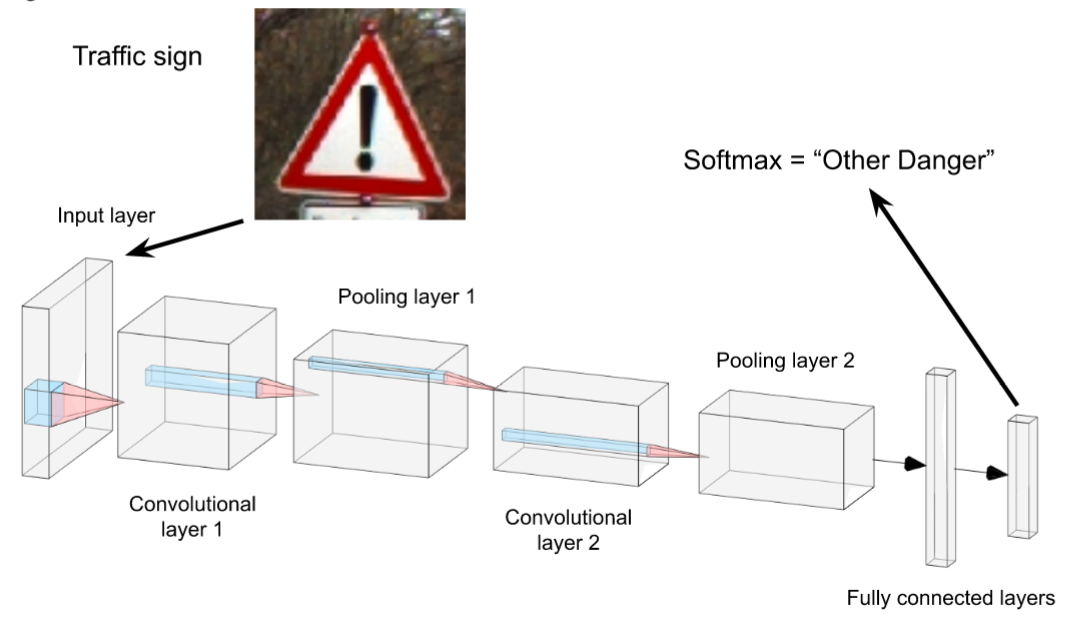
\includegraphics[width=0.8\textwidth]{Figs/APS360.png}
\end{center}
\caption{Example diagram of the architecture we will use to classify traffic signs. Exact architecture details may vary.}
\label{fig:CNN}
\end{figure}


\section{Architecture}
First, we will develop a classical ANN in order to compare its performance with the two baseline models. Implementing this first deep learning model will allow us to better understand the complexity of the data at our disposal, and the potential for underfitting and overfitting. This first model will lead to a phase of optimization of the hyperparameters in order to have the best performing model possible. 

Follow this a CNN will be implemented. The basic architecture for this CNN is outlined in Figure \ref{fig:CNN}. It is expected that the CNN will be more efficient than the ANN for image classification. The performance of this network will be tested on modified data (noise, rotation, zoom) in order to evaluate the robustness of the latter and perhaps to re-train it after a new and more advanced preprocessing phase.


Time permitting, we also intend to explore the use of autoencoders to combine this supervised learning task with unsupervised learning to increase the performance of the networks and to detect new features. Several architectures (encoders, convolutional or non convolutional autoencoders) could be tested in order to compare the performance of the latter in recognising patterns common to different labels.



\section{Baseline Model}
Having a baseline model is very important in order to have a reference against which to compare our performance metrics. The baseline is a very basic model to provide insight into the future performances of our models. Moreover, this simple model can be used to improve the understanding of our data. For example, we can find which class is easier to predict and which is harder, in order to maybe tune the prepossessing part.
We chose to start small and to use sklearn, which is a python library useful to implement in a very simple way a lot of machine learning algorithms. For classification problems, SVM (Support Vector Machine) and Decision Trees are commonly used.
SVM algorithms are effective in high dimensional space and could perform well for multiclass classification.
Decision trees are taking simple decision rules inferred from the data features. The results are simple to understand and interpret. However, decision trees can be unstable and can often overfit.
To observe the advantages of both algorithms, we will use them to have a first idea of how could simple machine learning algorithms can perform on the dataset used in this project. We will use the better model as our baseline for future comparisons.

\section{Ethical Considerations}
TSR systems are often used to aid decision making for self-driving cars. These autonomous driving systems have to take in a plethora of information and make driving decisions. Human lives are at stake considering the velocity cars move at and their overall size and weight \citep{9498342}. For example, if a self-driving car misclassified a stop sign, the car might drive through the intersection without stopping. This poses immense safety risks to other drivers and pedestrians. For this reason it is vital that machine learning algorithms can accurately make classifications with a high degree of confidence. 

From a theoretical standpoint, computers and machine learning algorithms should be be able to perform better than humans at driving, especially when considering how much information can be processed by a computer to make decisions in a short amount of time. However, within the scope of this project, if there is any uncertainty in the ability of a model to correctly classify a traffic sign, the safety risk of using machine learning to drive a car is too great compared to a human-driven vehicle \citep{9498342}. 

It is also imperative that data collection considered. Sign colours, styles, and appearances differ greatly from region to region across the globe. If models are trained on North American signs, the model may suffer when attempting to classify European signs which introduces safety risks that could come at the cost of human lives.

\section{Project Plan}
\label{ProjectPlan}
This section outlines our team's plan to manage our schedules and meet project deadlines. We will communicate asynchronously using the Discord messaging platform and meet regularly once a week during the 8pm lab period on Wednesdays. We will schedule additional meetings as needed, either in-person or over Discord. We have chosen to use Github to document the completion of work, make checkpoints of functioning code, and to mitigate the potential for code to be over-written.

All team members will be responsible for contributing to the project code, written reports, and final presentation. Table \ref{tab:task_table} provides an overview of the specific responsibilities of each team member and relevant deadlines. Additional tasks will be assigned when they arise, and tasks will be redistributed as needed to so that work is shared equally.

\begin{table}[t]
\caption{Responsibilities and internal deadlines}
\vspace{12pt}
\label{tab:task_table}
\resizebox{\textwidth}{!}{%
\begin{tabular}{lll}
\multicolumn{1}{c}{\bf TEAM MEMBER}  &\multicolumn{1}{c}{\bf RESPONSIBILITIES} &\multicolumn{1}{c}{\bf DEADLINE}
\\ \hline \\
\multirow{3}{*}{Arthur}    & • Setting up and managing Github                             & Oct 13 - initial setup                            \\
                           & • Basic code outline and structure                                        & Oct 22 - all major sections outlined              \\
                           & • Managing presentation slides                       & Nov 15 - presentation started                     \\\\
\multirow{3}{*}{Jordan}    & • Cleaning dataset     & Oct 22 - data cleaned for use by model            \\
                           & \multirow{2}{*}{• Obtaining model performance metrics}               & Oct 30 - metrics for progress report              \\
                           &                                                                           & Nov 26 - metrics for final report                 \\\\
\multirow{3}{*}{Katherine} & • Image pre-processing                                                    & Oct 23 - Pre-processing completed                 \\
                           & \multirow{2}{*}{• Latex document management} & Oct 23 - progress report started                  \\
                           &                                                                           & Nov 15 - final document started                   \\\\
\multirow{3}{*}{Mattéo}    & • Researching models for classification                                   & Oct 16 - list of models to implement              \\
                           & \multirow{2}{*}{• Hyperparameter optimization}                            & Oct 28 - parameters for progress report \\
                           &                                                                           & Nov 22 - parameters for final report   
\end{tabular}%
}
\end{table}

\section{Risk Register}
Below we have documented potential risks that our team has considered and courses of action that we will take should they occur.

\begin{enumerate}
\item A team member drops out of the course\begin{itemize}
\item In this situation we would immediately split up the assigned tasks of the group member who dropped amongst the remaining group members. This would be done considering the current workload and progress of each remaining team member. Additionally, we will try to split tasks based on familiarity and strengths of the remaining team members.
\end{itemize}
\item Our model takes too long to train \begin{itemize}
\item In this situation we find ourselves having to wait for significant amounts of time while training our model and are concerned about having results to evaluate. As a precautionary measure, we have adjusted our timeline in section~\ref{ProjectPlan} to give ourselves more time than we anticipate we'll need to train our model. Additionally, we plan to save checkpoints/instances of our model as we train it so that we can load a previous working version if training is taking too long. We also can simplify our model to make it train faster and sacrifice performance for results we can present and analyze at the end of the project
\end{itemize}
\item We realize there is too much data to work with \begin{itemize}
\item This situation could occur when we start looking deeper into our dataset and realize there is too much data to work with and it's making it too complicated to effectively train our model. In this case we plan to do more pre-processing of our data and reducing the sizes of our training, validation, and test datasets to a manageable size that we can work with. This can also shorten run-times.
\end{itemize}
\item A team member is unable to completely finish their portion of the project \begin{itemize}
\item This situation could occur when a team member gets overwhelmed, sick, or is otherwise unable to fulfil their responsibilities on the team for a period. We would redistribute the remaining tasks among the other team members to continue progressing on the project, similarly to the response if a team member had dropped the course. The difference in this situation is that as a team we would continue to check in with this team member to see how we can support them through the end of the project. Perhaps the team takes on more now and when the team member has more bandwidth later in the project they take on additional responsibilities. We will attempt to redistribute the tasks in such a way that there are still even contributions at the end of the project.
\end{itemize}
\item The code breaks right before the submission deadline \begin{itemize}
\item This situation could occur when we make a change close to the deadline and our code no longer works as intended or "breaks" and can no longer run at all. As a precautionary measure, we have chosen to store our code on GitHub, a version control system for code. This way we can revert back to the last known working version of our code and not have to worry about wasting time trying to chase down a bug that broke our code. Additionally, we will also document our progress so we can quickly identify the last known working version and know details about that version should we have to use it under a time crunch.
\end{itemize}
\end{enumerate}

\section{Link to GitHub}
Our project repository can be found at the following link:
\begin{center}
    \url{https://github.com/Arthur-Akb/GTSRB-APS360-Project}
\end{center}
\label{last_page}

\bibliography{APS360_ref}
\bibliographystyle{iclr2022_conference}

\end{document}





\begin{figure}[h]
\begin{center}

\includegraphics[width=0.6\textwidth]{Figs/td-deep-learning.jpg}
\end{center}
\caption{Sample figure caption. Image: ZDNet}
\end{figure}



\subsection{Tables}

All tables must be centered, neat, clean and legible. Do not use hand-drawn
tables. The table number and title always appear before the table. See
Table~\ref{sample-table}.

Place one line space before the table title, one line space after the table
title, and one line space after the table. The table title must be lower case
(except for first word and proper nouns); tables are numbered consecutively.

\begin{table}[t]
\caption{Sample table title}
\label{sample-table}
\begin{center}
\begin{tabular}{ll}
\multicolumn{1}{c}{\bf PART}  &\multicolumn{1}{c}{\bf DESCRIPTION}
\\ \hline \\
Dendrite         &Input terminal \\
Axon             &Output terminal \\
Soma             &Cell body (contains cell nucleus) \\
\end{tabular}
\end{center}
\end{table}


\section{Default Notation}

In an attempt to encourage standardized notation, we have included the
notation file from the textbook, \textit{Deep Learning}
\cite{goodfellow2016deep} available at
\url{https://github.com/goodfeli/dlbook_notation/}.  Use of this style
is not required and can be disabled by commenting out
\texttt{math\_commands.tex}.


\centerline{\bf Numbers and Arrays}
\bgroup
\def\arraystretch{1.5}
\begin{tabular}{p{1in}p{3.25in}}
$\displaystyle a$ & A scalar (integer or real)\\
$\displaystyle \va$ & A vector\\
$\displaystyle \mA$ & A matrix\\
$\displaystyle \tA$ & A tensor\\
$\displaystyle \mI_n$ & Identity matrix with $n$ rows and $n$ columns\\
$\displaystyle \mI$ & Identity matrix with dimensionality implied by context\\
$\displaystyle \ve^{(i)}$ & Standard basis vector $[0,\dots,0,1,0,\dots,0]$ with a 1 at position $i$\\
$\displaystyle \text{diag}(\va)$ & A square, diagonal matrix with diagonal entries given by $\va$\\
$\displaystyle \ra$ & A scalar random variable\\
$\displaystyle \rva$ & A vector-valued random variable\\
$\displaystyle \rmA$ & A matrix-valued random variable\\
\end{tabular}
\egroup
\vspace{0.25cm}
\centerline{\bf Sets and Graphs}
\bgroup
\def\arraystretch{1.5}

\begin{tabular}{p{1.25in}p{3.25in}}
$\displaystyle \sA$ & A set\\
$\displaystyle \R$ & The set of real numbers \\
$\displaystyle \{0, 1\}$ & The set containing 0 and 1 \\
$\displaystyle \{0, 1, \dots, n \}$ & The set of all integers between $0$ and $n$\\
$\displaystyle [a, b]$ & The real interval including $a$ and $b$\\
$\displaystyle (a, b]$ & The real interval excluding $a$ but including $b$\\
$\displaystyle \sA \backslash \sB$ & Set subtraction, i.e., the set containing the elements of $\sA$ that are not in $\sB$\\
$\displaystyle \gG$ & A graph\\
$\displaystyle \parents_\gG(\ervx_i)$ & The parents of $\ervx_i$ in $\gG$
\end{tabular}
\vspace{0.25cm}


\centerline{\bf Indexing}
\bgroup
\def\arraystretch{1.5}

\begin{tabular}{p{1.25in}p{3.25in}}
$\displaystyle \eva_i$ & Element $i$ of vector $\va$, with indexing starting at 1 \\
$\displaystyle \eva_{-i}$ & All elements of vector $\va$ except for element $i$ \\
$\displaystyle \emA_{i,j}$ & Element $i, j$ of matrix $\mA$ \\
$\displaystyle \mA_{i, :}$ & Row $i$ of matrix $\mA$ \\
$\displaystyle \mA_{:, i}$ & Column $i$ of matrix $\mA$ \\
$\displaystyle \etA_{i, j, k}$ & Element $(i, j, k)$ of a 3-D tensor $\tA$\\
$\displaystyle \tA_{:, :, i}$ & 2-D slice of a 3-D tensor\\
$\displaystyle \erva_i$ & Element $i$ of the random vector $\rva$ \\
\end{tabular}
\egroup
\vspace{0.25cm}


\centerline{\bf Calculus}
\bgroup
\def\arraystretch{1.5}
\begin{tabular}{p{1.25in}p{3.25in}}
% NOTE: the [2ex] on the next line adds extra height to that row of the table.
% Without that command, the fraction on the first line is too tall and collides
% with the fraction on the second line.
$\displaystyle\frac{d y} {d x}$ & Derivative of $y$ with respect to $x$\\ [2ex]
$\displaystyle \frac{\partial y} {\partial x} $ & Partial derivative of $y$ with respect to $x$ \\
$\displaystyle \nabla_\vx y $ & Gradient of $y$ with respect to $\vx$ \\
$\displaystyle \nabla_\mX y $ & Matrix derivatives of $y$ with respect to $\mX$ \\
$\displaystyle \nabla_\tX y $ & Tensor containing derivatives of $y$ with respect to $\tX$ \\
$\displaystyle \frac{\partial f}{\partial \vx} $ & Jacobian matrix $\mJ \in \R^{m\times n}$ of $f: \R^n \rightarrow \R^m$\\
$\displaystyle \nabla_\vx^2 f(\vx)\text{ or }\mH( f)(\vx)$ & The Hessian matrix of $f$ at input point $\vx$\\
$\displaystyle \int f(\vx) d\vx $ & Definite integral over the entire domain of $\vx$ \\
$\displaystyle \int_\sS f(\vx) d\vx$ & Definite integral with respect to $\vx$ over the set $\sS$ \\
\end{tabular}
\egroup
\vspace{0.25cm}

\centerline{\bf Probability and Information Theory}
\bgroup
\def\arraystretch{1.5}
\begin{tabular}{p{1.25in}p{3.25in}}
$\displaystyle P(\ra)$ & A probability distribution over a discrete variable\\
$\displaystyle p(\ra)$ & A probability distribution over a continuous variable, or over
a variable whose type has not been specified\\
$\displaystyle \ra \sim P$ & Random variable $\ra$ has distribution $P$\\% so thing on left of \sim should always be a random variable, with name beginning with \r
$\displaystyle  \E_{\rx\sim P} [ f(x) ]\text{ or } \E f(x)$ & Expectation of $f(x)$ with respect to $P(\rx)$ \\
$\displaystyle \Var(f(x)) $ &  Variance of $f(x)$ under $P(\rx)$ \\
$\displaystyle \Cov(f(x),g(x)) $ & Covariance of $f(x)$ and $g(x)$ under $P(\rx)$\\
$\displaystyle H(\rx) $ & Shannon entropy of the random variable $\rx$\\
$\displaystyle \KL ( P \Vert Q ) $ & Kullback-Leibler divergence of P and Q \\
$\displaystyle \mathcal{N} ( \vx ; \vmu , \mSigma)$ & Gaussian distribution %
over $\vx$ with mean $\vmu$ and covariance $\mSigma$ \\
\end{tabular}
\egroup
\vspace{0.25cm}

\centerline{\bf Functions}
\bgroup
\def\arraystretch{1.5}
\begin{tabular}{p{1.25in}p{3.25in}}
$\displaystyle f: \sA \rightarrow \sB$ & The function $f$ with domain $\sA$ and range $\sB$\\
$\displaystyle f \circ g $ & Composition of the functions $f$ and $g$ \\
  $\displaystyle f(\vx ; \vtheta) $ & A function of $\vx$ parametrized by $\vtheta$.
  (Sometimes we write $f(\vx)$ and omit the argument $\vtheta$ to lighten notation) \\
$\displaystyle \log x$ & Natural logarithm of $x$ \\
$\displaystyle \sigma(x)$ & Logistic sigmoid, $\displaystyle \frac{1} {1 + \exp(-x)}$ \\
$\displaystyle \zeta(x)$ & Softplus, $\log(1 + \exp(x))$ \\
$\displaystyle || \vx ||_p $ & $\normlp$ norm of $\vx$ \\
$\displaystyle || \vx || $ & $\normltwo$ norm of $\vx$ \\
$\displaystyle x^+$ & Positive part of $x$, i.e., $\max(0,x)$\\
$\displaystyle \1_\mathrm{condition}$ & is 1 if the condition is true, 0 otherwise\\
\end{tabular}
\egroup
\vspace{0.25cm}


